\documentclass[dvipdfmx,titlepage,a4j]{jsarticle}

\usepackage{url}
\usepackage{graphicx}
\usepackage{listings,jvlisting}
\usepackage{amsmath,amssymb}
\usepackage{graphicx}
\usepackage[yen]{okuverb}
\usepackage{ascmac}
\usepackage{fancybox}
\usepackage{fancyvrb}
\usepackage{fancyhdr}
\usepackage{lastpage}
\usepackage{caption}
\usepackage{subcaption}
\usepackage{here}

\fancypagestyle{foot}
{
\fancyhead[C]{}
\fancyfoot[C]{\thepage / \pageref{LastPage}}
\renewcommand\headrulewidth{0.4pt}
}

%ここからソースコードの表示に関する設定
\lstset{
  language={C++},
  basicstyle={\ttfamily},
  identifierstyle={\small},
  commentstyle={\smallitshape},
  keywordstyle={\small\bfseries},
  ndkeywordstyle={\small},
  stringstyle={\small\ttfamily},
  frame={tb},
  tabsize={2},
  breaklines=true,
  columns=[l]{fullflexible},
  numbers=left,
  xrightmargin=0zw,
  xleftmargin=3zw,
  numberstyle={\scriptsize},
  stepnumber=1,
  numbersep=1zw,
  lineskip=-0.5ex
}

\title{タイトル}
\author{waarrk}
\date{2023年2月1日}

\begin{document}

\begin{titlepage}
    \centering
    \vspace*{2cm}

    \vspace{1cm}

    {\LARGE \textbf{主成分分析によるIrisデータセットの解析}}

    \vspace{0.5cm}

    {\LARGE 2024年度開講 数値解析学レポート}

    \vspace{1.5cm}

    {\textbf{千葉工業大学 先進工学部 未来ロボティクス学科}\\}
    {\textbf{22C1704 鷲尾 優作}}

    \vfill

    {\large 2024年7月25日}

    \vspace{1cm}
\end{titlepage}

\section{目的}
本稿では、アヤメの花のデータセットであるIrisデータセットのうち、品種別データに
対して主成分分析を行い、データの解析手法を学ぶことを目的とする.

\section{理論}

主成分分析(PCA)は、多次元データの次元削減を行うための統計手法である.PCAの目的は、データの分散を最大化する方向(主成分)を見つけ出し、元のデータを少数の主成分に変換することで、データの特徴を効果的に表現することである.PCAは以下のステップで実施される:

\begin{enumerate}
    \item \textbf{データの標準化}:各変数を平均0、分散1に標準化し、スケールの違いによる影響を排除する.
    \item \textbf{共分散行列の計算}:標準化したデータから共分散行列を計算し、変数間の関係性を把握する.
    \item \textbf{固有ベクトルと固有値の計算}:共分散行列の固有ベクトルと固有値を求め、主成分の方向とその重要性を評価する.
    \item \textbf{主成分の選択}:固有値に基づき、主要な主成分を選択し、データをその主成分に投影して次元削減を行う.
    \item \textbf{データの変換}:元のデータを選択した主成分に投影し、次元削減されたデータを得る.
\end{enumerate}

\subsection{問題設定}

次の問題設定に基づいて、主成分分析を行う:

\begin{itemize}
    \item \textbf{データセット}:Irisデータセット(アヤメの3種類の品種に関する花弁とがく片の長さと幅のデータ)
    \item \textbf{目標}:データの次元を削減し、各品種が主成分空間でどのように分布しているかを視覚化する.
    \item \textbf{次元削減}:元の4次元の特徴量から、2次元の主成分に次元削減を行う.
\end{itemize}

\subsection{評価方法}

主成分分析の結果を定量的に評価するために、以下の指標を用いる:

\begin{enumerate}
    \item \textbf{分散説明率}:各主成分がデータの総分散に対してどの程度寄与しているかを示す指標であり、主成分の重要性を評価する.累積分散説明率も併せて確認し、次元削減の効果を評価する.
    \item \textbf{主成分の可視化}:主成分分析によって得られた主成分空間におけるデータポイントの分布をプロットし、異なるクラス(品種)の分布の明確さを評価する.特に、品種ごとに色分けし、主成分空間での分離具合を確認する.
    \item \textbf{再構成誤差}:データを主成分空間に投影した後、元の空間に再構成し、元データと再構成データとの差を計測する.これにより、次元削減による情報損失を評価する.
\end{enumerate}

\section{シミュレーション結果}

シミュレーションの結果を以下に示す.図\ref{fig:sim}に、主成分分析によって次元削減されたデータの状態遷移と観測の変化をグラフ化して示す.

図\ref{fig:sim}は、主成分分析によって得られた2次元の主成分空間におけるデータポイントの分布を示している.元の4次元の特徴量が2次元の主成分に投影され、各アヤメの品種(Setosa、Versicolor、Virginica)が異なる色で表示されている.これにより、品種ごとのデータの分布状況と、主成分空間での分離度合いを視覚的に確認することができる.

具体的には、以下の点が図\ref{fig:sim}から読み取れる.
\begin{itemize}
    \item \textbf{品種間の分離}:主成分空間において、Setosaは他の2品種(Versicolor、Virginica)とは明確に分離している.主成分分析が品種間の違いを効果的に捉えていることが確認できる.VersicolorとVirginicaのデータポイントは部分的に重なり合っているが、主成分空間内で一定のクラスタリングが観察できる.
    \item \textbf{データの分布}:主成分空間における各品種のデータポイントの密度や分布状況から、品種ごとのデータの集中度や分散状況が確認できる.これにより、次元削減による情報の保持とデータの可視化の有効性が評価できる.
\end{itemize}

分散説明率に関する具体的な結果は以下の通りである.
\begin{itemize}
    \item \textbf{分散説明率(各主成分)}:主成分1が約72.96\%、主成分2が約22.85\%の分散を説明している.
    \item \textbf{累積分散説明率}:主成分1と主成分2を合わせると、データ全体の約95.81\%の分散を説明している.
\end{itemize}

再構成誤差は約0.0418であり、次元削減後のデータと再構成データとの差が比較的小さいことを示している.

\begin{figure}[H]
    \centering
    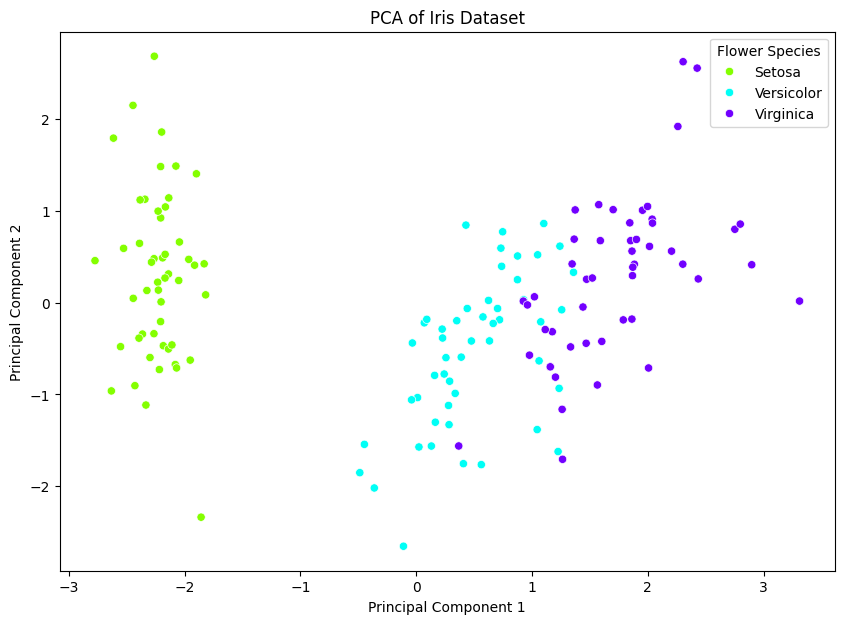
\includegraphics[width=0.7\textwidth]{picture/sim.png}
    \caption{PCAによるIrisデータセットの主成分空間での可視化}
    \label{fig:sim}
\end{figure}

\section{考察}

主成分分析の結果は、Irisデータセットに対して次元削減が効果的であることを示している.特に、主成分分析を用いることで、元の4次元の特徴量から2次元の主成分空間に次元削減する際に、各品種のデータが明確に分離されることが確認できた.
具体的には、図\ref{fig:sim}に示されたように、Setosaは他の2品種(Versicolor、Virginica)とは明確に分離している.このことから、主成分分析がSetosaと他の品種との違いを効果的に捉えていることがわかる.主成分空間におけるSetosaのデータポイントは、他の品種と比較して分布が一貫しており、次元削減によって得られた主成分が品種の識別に有効であることが示されている.
一方で、VersicolorとVirginicaのデータポイントは部分的に重なり合っていることから、
主成分分析が全ての品種の違いを完全に分離できるわけではないことがわかる.
主成分分析はデータの分散を最大化する方向を見つけるが、すべての品種間の違いを完全に捉えることができるわけではない.
したがって、さらなる解析や他の次元削減手法を併用することで、より精度の高い識別が可能となると考えられる.

分散説明率の結果は、主成分1と主成分2がデータの約95.81\%の分散を説明しており、
主成分分析がデータの主要な情報を効果的に捉えていることを示している.再構成誤差が約0.0418であることから、次元削減後のデータと再構成データとの差が比較的小さいことが確認され、
次元削減による情報の損失が限定的であることが示されている.

\section{付録}
\subsection{シミュレーションプログラム}

\lstinputlisting[caption=sim.png,label=prog:sim]{program/sim.py}

\nocite{*}
\bibliographystyle{jplain}
\bibliography{refs}

\end{document}
